% The Slide Definitions
%document
\documentclass[10pt]{beamer}
%theme
\usetheme{metropolis}
% packages
\usepackage{color}
\usepackage{listings}
\usepackage[ngerman]{babel}
\usepackage[utf8]{inputenc}
\usepackage{multicol}


% color definitions
\definecolor{mygreen}{rgb}{0,0.6,0}
\definecolor{mygray}{rgb}{0.5,0.5,0.5}
\definecolor{mymauve}{rgb}{0.58,0,0.82}

\lstset{
    backgroundcolor=\color{white},
    % choose the background color;
    % you must add \usepackage{color} or \usepackage{xcolor}
    basicstyle=\footnotesize\ttfamily,
    % the size of the fonts that are used for the code
    breakatwhitespace=false,
    % sets if automatic breaks should only happen at whitespace
    breaklines=true,                 % sets automatic line breaking
    captionpos=b,                    % sets the caption-position to bottom
    commentstyle=\color{mygreen},    % comment style
    % deletekeywords={...},
    % if you want to delete keywords from the given language
    extendedchars=true,
    % lets you use non-ASCII characters;
    % for 8-bits encodings only, does not work with UTF-8
    frame=single,                    % adds a frame around the code
    keepspaces=true,
    % keeps spaces in text,
    % useful for keeping indentation of code
    % (possibly needs columns=flexible)
    keywordstyle=\color{blue},       % keyword style
    % morekeywords={*,...},
    % if you want to add more keywords to the set
    numbers=left,
    % where to put the line-numbers; possible values are (none, left, right)
    numbersep=5pt,
    % how far the line-numbers are from the code
    numberstyle=\tiny\color{mygray},
    % the style that is used for the line-numbers
    rulecolor=\color{black},
    % if not set, the frame-color may be changed on line-breaks
    % within not-black text (e.g. comments (green here))
    stepnumber=1,
    % the step between two line-numbers.
    % If it's 1, each line will be numbered
    stringstyle=\color{mymauve},     % string literal style
    tabsize=4,                       % sets default tabsize to 4 spaces
    % show the filename of files included with \lstinputlisting;
    % also try caption instead of title
    language = [Sharp]C,
	showspaces = false,
	showtabs = false,
	showstringspaces = false,
	escapechar = ,
}

\def\ContinueLineNumber{\lstset{firstnumber=last}}
\def\StartLineAt#1{\lstset{firstnumber=#1}}
\let\numberLineAt\StartLineAt



\newcommand{\codeline}[1]{
	\alert{\texttt{#1}}
}


% Author and Course information
% This Document contains the information about this course.

% Authors of the slides
\author{\href{https://github.com/evilham}{@evilham}\\
\footnotesize{Basierend auf Folien von \href{https://github.com/satkowski}{@satkowski} (November 2016)}}

% Name of the Course
\institute{C\texttt{\#} Kurs}

% Fancy Logo
\titlegraphic{\hfill
\includegraphics[height=1.25cm]{../templates/fsr_logo_cropped}}


% Presentation title
\title{Grundlagen von C\texttt{\#} - 1 (Zusammenfassung)}
\date{\today}

\usepackage{subfig}
\begin{document}

\maketitle

% ----------------------- Über den Kurs ------------------------------
\begin{frame}{Über diesen Kurs}
	\centering 11 Kurseinheiten und viele Aufgaben.
	
	Ostern wird über das Semester nachgeholt.
	
	\vspace{0.7cm}
	\centering Die Materialien findet ihr hier:
	
	\huge \href{https://evilham.com/csharp2017}{evilham.com/csharp2017}

\end{frame}

% ----------------------- Warum C#? ------------------------------
\begin{frame}{Warum C\texttt{\#} und wohin?}
C\texttt{\#} kann alles! Einige Möglichkeiten:
\begin{itemize}
\item Autodesk \href{https://en.wikipedia.org/wiki/AutoCAD}{AutoCAD}, \href{https://en.wikipedia.org/wiki/Revit}{Revit} Plugins Entwicklung
\item \href{https://dev.office.com/}{Microsoft Office} Plugins Entwicklung
\item Desktop GUI Programmierung mit \href{https://en.wikipedia.org/wiki/Windows_Forms}{Windows Forms} oder \href{http://www.wpf-tutorial.com/about-wpf/what-is-wpf/}{WPF}
\item \href{https://en.wikipedia.org/wiki/Network_socket}{Netzwerk Protokolle} mit reinem C\texttt{\#}
\item Webserver Programmierung mit \href{https://www.asp.net/}{ASP.net}
\item Android Programmierung mit \href{https://en.wikipedia.org/wiki/Xamarin}{Xamarin}
\item Cross-Platform Entwicklung mit \href{https://dot.net}{.Net Core}
\end{itemize}
\end{frame}

\begin{frame}{Autodesk? AutoCAD? Revit?}
\href{https://en.wikipedia.org/wiki/Autodesk}{Autodesk} ist eine Avantgarde Software Firma, ihr Software wird in viele Bereichen verwendet: Architektur, Maschinenbau, Hoch- und Tiefbau, Filmindustrie, Automotive...

Erweiterungssoftware für \alert{AutoCAD} oder \alert{Revit} ist immer in Nachfrage.

\begin{figure}
    \centering
    \subfloat[\href{https://twitter.com/AutoCAD/status/857685795376959492}{Infrastruktur}]{{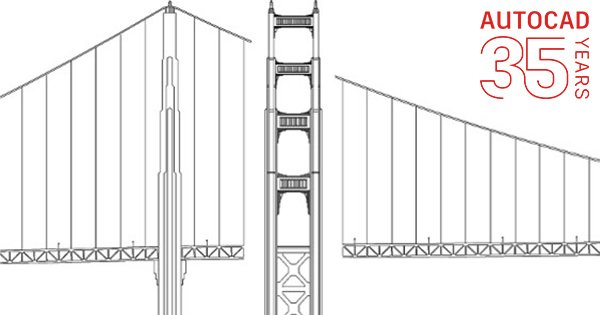
\includegraphics[width=5cm]{resources/01_grundlagen_1/autocad1.jpg} }}
    \qquad
    \subfloat[\href{https://twitter.com/AutoCAD/status/854020636351582209}{Maschinenbau}]{{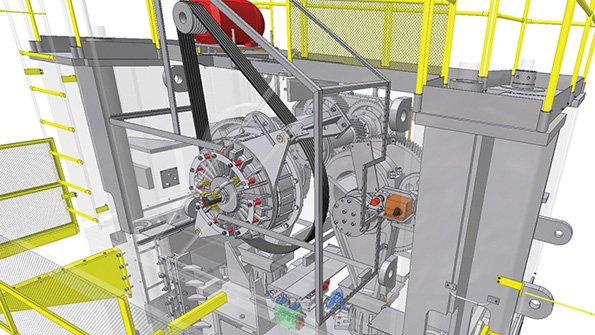
\includegraphics[width=5cm]{resources/01_grundlagen_1/autocad2.jpg} }}%
    \caption{Things done with Autodesk's products\\
    (Source: \href{https://twitter.com/autocad}{https://twitter.com/autocad})}%
    \label{fig:example}
\end{figure}

\end{frame}

% ----------------------- Erinnerung -----------------------------
\begin{frame}{Hello World}
    \lstinputlisting{resources/01_grundlagen_1/zusammenfassung.cs}
\end{frame}
\end{document}